%! TEX ROOT = ./main.tex

\section{Introduction}

Synthesizing formally verified controllers for safety-critical dynamical systems has emerged as an important problem.
The goal is to algorithmically synthesize controllers so that the systems under control only do what they are meant to do, even in the presence of external disturbances.
One such algorithmic technique is the so-called Abstraction-Based Controller Design (ABCD).
In ABCD, we start with a model of a continuous nonlinear dynamical system and a control task.
The sought controller is synthesized in three stages:
First, we approximate the continuous system model using a finite state abstraction.
Second, we compute an abstract controller for the abstraction by using reactive synthesis techniques.
Third, we refine the abstract controller to the sought final controller for the continuous system.
The desired correctness guarantee of the obtained controller follows from a careful abstraction construction process.

The strengths of ABCD are its versatility: 
It can handle arbitrary continuous nonlinear system models, external disturbances, modeling uncertainties, measurement errors, $\omega$-regular control specifications, and so on.
The weakness of ABCD is its poor scalability: 
Usually ABCD uses a state-space discretization for computing the abstraction, which causes an exponential blow-up in the time and space complexity.

In this paper, we extend ABCD---more in a practical sense---to synthesize controllers for a group of robots, operating in a shared workspace.
Suppose, we have a group of robots which have been assigned a joint \emph{reach-avoid} task, where the robots need to collectively reach a set of target states while collectively avoiding a set of static obstacles.
The joint task might need the robots to coordinate their actions among each other.
For example, if two robots need to jointly carry a heavy object from one place to another without letting the object fall, they need to move in perfect harmony.

Perhaps the most straightforward solution approach will be to use a centralized approach, by treating the group of robots as one single system.
In the centralized approach, we need to build a product of the models of the robots; the product captures the simultaneous evolution of the global state of the system.
Then, in theory, we can apply ABCD on the product to synthesize a global controller for the robots.
Unfortunately, the centralized approach will not be practical, because ABCD would not scale to the potentially large size of the product state space.

On the other hand, a purely decentralized synthesis, where we compute controller for each robot in isolation, is also challenging.
Usually, decentralized synthesis requires each robot to treat the other robots as adversaries, to account for the worst-case scenarios.
This is a very strong assumption, and often we will not get any controller.
For instance, recall the example of two robots jointly carrying an object.
There each of the robots will need to assume that the other robot will do everything to run away and make the object fall, which is an unrealistically strong assumption.

To circumvent these issues, in this paper, we propose a \emph{semi-centralized} and \emph{hierarchical} synthesis approach, which will give us decentralized controllers for the joint task.
In the top level, we use the centralized method with a fast synthesis tool to make a joint global plan.
In this paper, we use ALTRO \cite{howell2019altro}, which is an optimal control-based controller synthesis tool that scales quite well to large dimensional systems.
ALTRO does not provide formal guarantees against external disturbances or modeling uncertainties.
So in the bottom level, first we decompose the global plan into local plans for each robot, and then use ABCD to locally synthesize formally verified controllers to track the local plans.
(The decomposition is straightforward, because ALTRO gives us a central open-loop controller.)
Our approach is modular:
We could replace ALTRO with any other fast and scalable method, and we could replace ABCD with any other suitable method that provides guarantees, and we would still get the formally verified decentralized controllers for the robots.

We demonstrate the usefulness of our approach using several multi-robot controller synthesis examples.



\begin{comment}
The collision avoidance requirement, in the absence of inter-robot communication, makes the decentralized controller synthesis problem especially challenging.
One option will be to treat the other robots as dynamic obstacles.
There are two problems.
Firstly, it is not known how to deal with dynamic obstacles in the ABCD framework.
Secondly, even if we knew how to deal with that, this dynamic obstacle assumption could lead to pessimistic, and often empty, solution.

On the other hand, the issue with dynamic obstacles goes away if we use a centralized approach, by treating the group of robots as one single system.
In the centralized approach, we need to build a product of the models of each individual robot; the product captures the simultaneous evolution of the global state of the system.
The states of collision, which are dynamic in nature, now conveniently become a set of static obstacles in the global state space.
We can then, at least in theory, use ABCD to synthesize a joint controller for the group of robots, and afterwards decompose the joint controller into individual controller for each robot.
(The decomposition is possible due to the underlying decentralized control structure.)

Unfortunately, ABCD does not scale to the usual large size of the global state space in the centralized approach.
To circumvent this issue, in this paper, we propose a two-layered hierarchical controller synthesis approach involving ABCD.
In the top layer, we use some off-the-shelf fast controller synthesis method to make a joint global plan using the aforementioned centralized approach.
In this paper, we use ALTRO \cite{howell2019altro} in the top layer, which is an optimal-control-based controller synthesis tool that scales quite well to large dimensional system.
Unfortunately, the fast and scalable tools, including ALTRO, usually do not provide formal guarantees against external disturbances or modeling uncertainties.
So in the bottom layer, we use ABCD to synthesize formally verified \emph{tracking} controller for each robot for following the projection of the joint plan on the robot's state space.
\end{comment}



\subsection{Motivating Example}

Consider a multi-robot reach-avoid problem in a factory setting:
We have an overhead crane hanging from a trolley which runs along an overhead horizontal rail; the crane is modeled as a pendulum and the trolley as an one-dimensional cart.
We also have a factory vehicle that drives underneath the crane, in the same horizontal axis as the overhead rail.
Suppose, when the crane is in the vertically downward position, it obstructs the vehicle's movement.
The scenario is illustrated in Fig.~\ref{fig:cr_and_lft} (\textbf{left}); the four different subfigures from top to bottom will be referred to as Frame~1-4 respectively.

Initially the crane is resting in its vertically downward position at the leftmost point along the rail, and the vehicle is positioned at the rightmost point (Frame~1).
Suppose in the end, they need to reach the configuration shown in Frame~4, i.e., they need to cross each other while maintaining a minimum safe distance.
To make this possible, the trolley needs to accelerate enough to swing the crane up (Frame~2-3) and create sufficient room for the vehicle to pass.
When the crane swings up high enough, the vehicle must make a timely and swift passage before the crane comes down due to gravity.
We want to design a pair of controllers, one for the trolley and one for the vehicle, which will execute this joint maneuver.

Suppose, both the vehicle and the crane are subjected to disturbances, representing (a) external factors like wind for the crane and slippery floor for the vehicle, and (b) modeling imperfections.
We want the controllers to be robust against the worst-case disturbances to the system.
In reality, worst-case disturbances might well be rare events, but safeguarding against them will certify absolute correctness.

Since we do not assume any run-time communication between the controllers, a completely decentralized synthesis would be difficult.
One option would be to assume the worst-case behavior of the other system, and attempt to achieve the goal.
This might be too restrictive:
For instance, with this assumption, the vehicle will not be able to achieve it's goal, because the crane can choose to stay down all the time.

To alleviate this issue, we employ a semi-centralized hierarchical synthesis approach.
At the \textbf{top level} of the hierarchical approach, we ignore the disturbances, and treat the crane and the vehicle as one joint system, called the \emph{product system}.
Next, we use a \emph{planner} to obtain a \emph{global} open-loop controller for the product system.
(An open-loop controller is one that bases its control decision on the current time instant.)
Among the existing off-the-shelf planning tools we selected ALTRO which is a scalable and fast controller synthesis tool that is suitable for the possibly high dimension of the product system.

Since the obtained controller is open-loop, hence we can easily decompose the central controller into individual open-loop controllers---called \emph{local} open-loop controllers---for the crane and the vehicle.
However, there will be no guarantee that the local open-loop controllers will fulfill the specification when the disturbances come into effect.
Actually, Fig.~\ref{fig:cr_and_lft}, (\textbf{left}) shows various moments in the simulation of the local open-loop controllers in the absence of the disturbances, and Frame~3 shows that the crane and vehicle get very close to eachother. However, in the presence of disturbances the crane and vehicle can collide as the constraint of the minimum safe distance is violated (Fig.~\ref{fig:cr_and_lft}, (\textbf{right})). 

To deal with this robustness issue, at the \textbf{bottom level} of our hierarchical approach, we employ a \emph{guaranteed tracking method} to ``robustify'' the local open-loop controllers against disturbances.
Our choice to achieve guaranteed tracking is ABCD. More concretely, we consider the open-loop controlled trajectory of \emph{each system in isolation}, and use ABCD to synthesize a \emph{tracking controller}.
The goal of the tracking controller is to track the open-loop trajectories within some small neighborhood, even in the presence of worst-case disturbances.
ABCD gives us the sought \emph{local feedback controller} for each individual system.

%\begin{figure}[t]
%	\centering
%	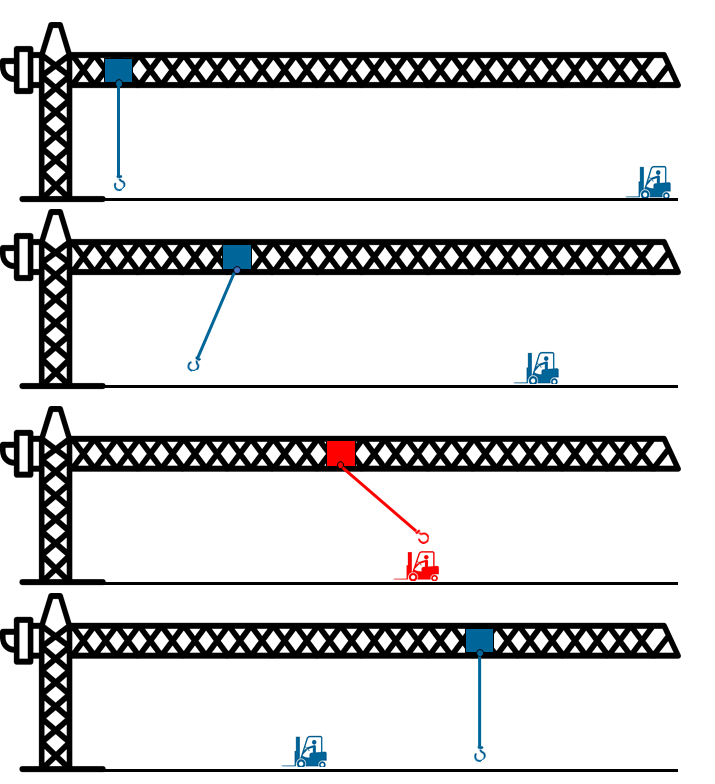
\includegraphics[width=0.45\textwidth]{figures/crane_and_lifter.png}
%	\caption{Illustration of the reference trajectories produced by the open-loop planner for the crane and the factory vehicle example}
%	\label{fig:cr_and_lft}
%\end{figure}
\begin{figure}[t]
	\centering
	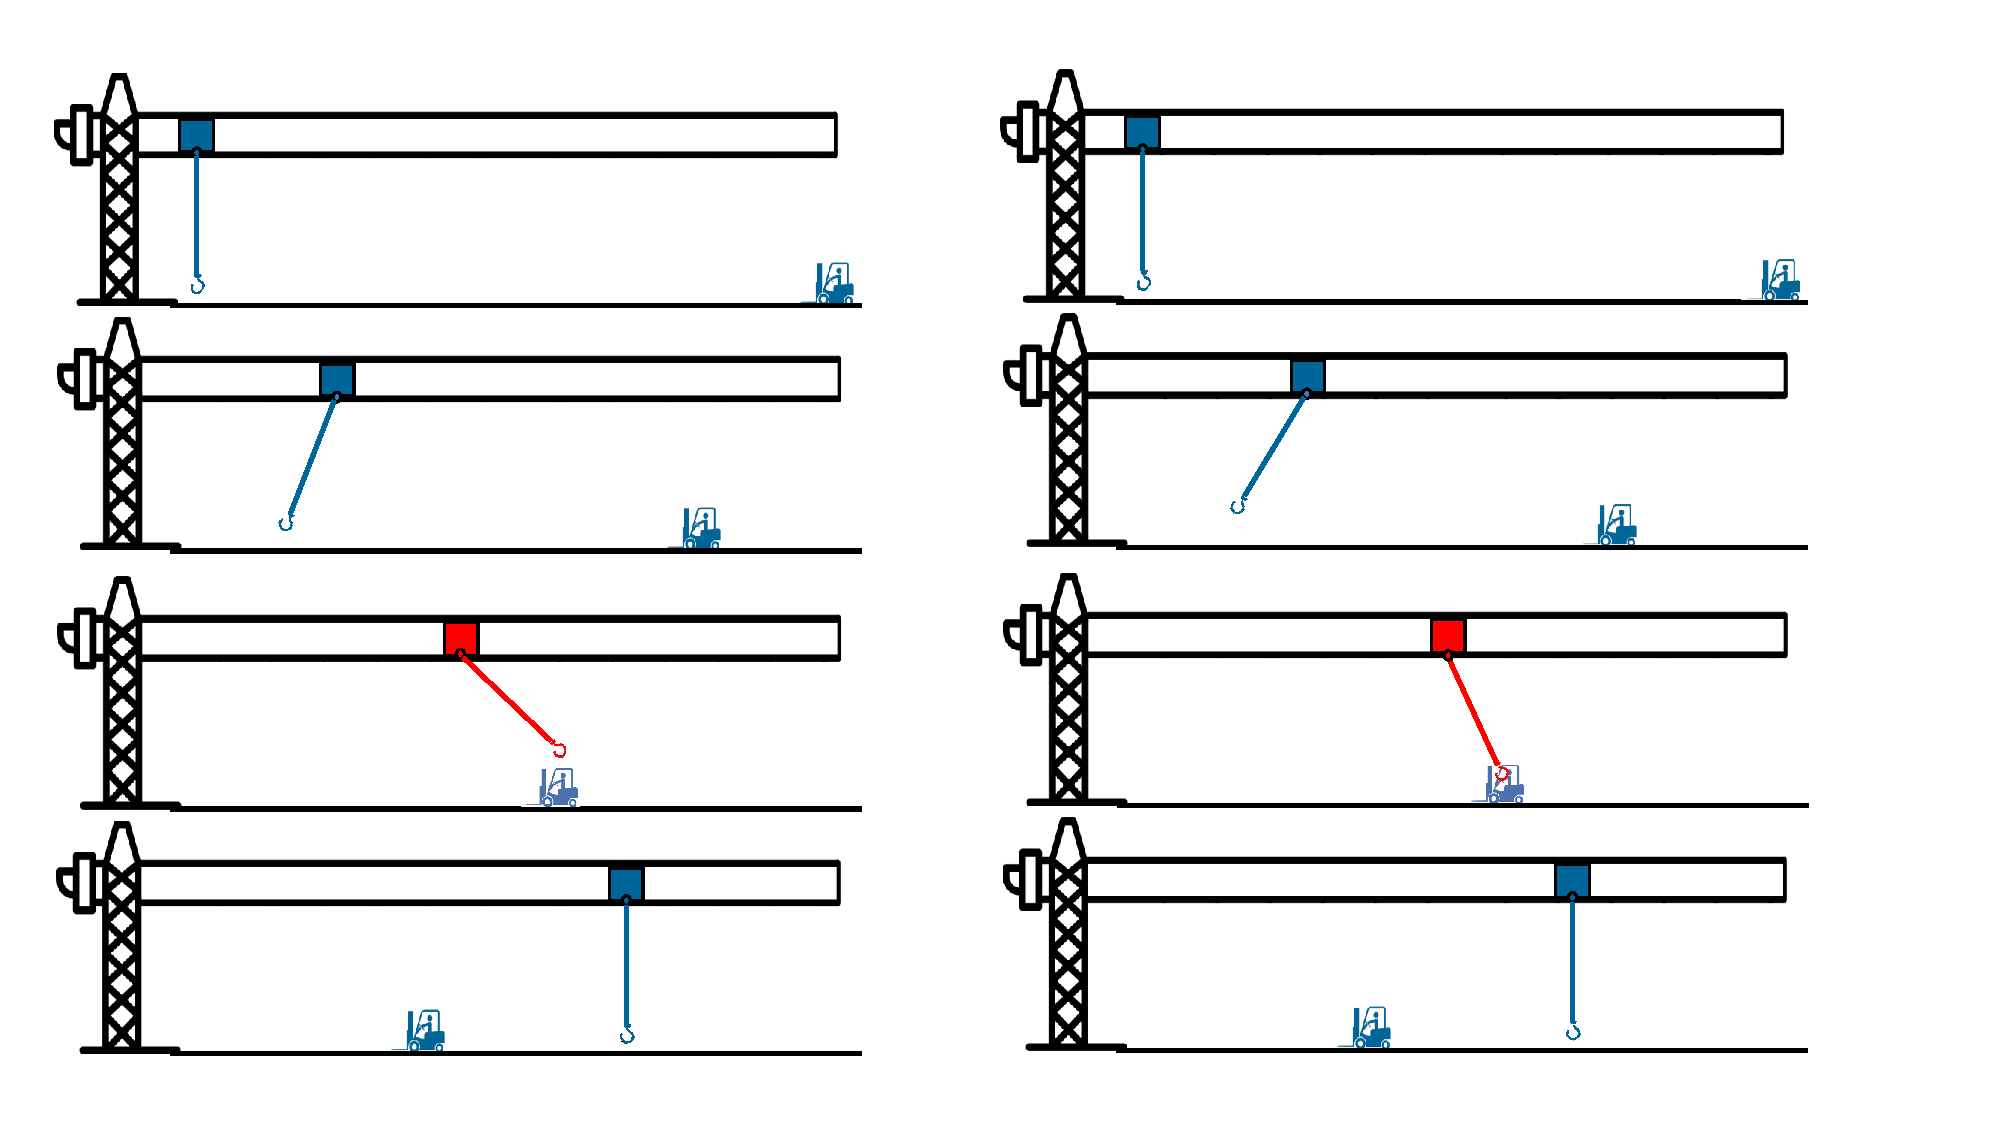
\includegraphics[width=0.5\textwidth]{figures/crane_and_forklifter.pdf}
	\caption{Illustration of the trajectories generated by the open-loop controller for the crane and vehicle example under disturbance-free (\textbf{left}) and perturbed (\textbf{right}) situations} 
	\label{fig:cr_and_lft}
\end{figure}
